\documentclass{article}
\usepackage[left=0.85in, right=0.85in, top=0.5in, bottom=0.95in]{geometry}
\usepackage[T1]{fontenc}
\usepackage[utf8]{inputenc}
\usepackage[italian]{babel}
\usepackage{graphicx}
\usepackage{wrapfig2}
\usepackage{amsmath}
\usepackage{amsthm} %teoremi e dimostrazioni
\usepackage{amssymb}
\usepackage{cases}
\usepackage{subcaption}
\usepackage{hyperref}
\hypersetup{
	colorlinks=true,
	linkcolor=blue,    
	urlcolor=blue,
	pdfpagemode=FullScreen,
}
\urlstyle{same}
\usepackage{changepage}
\usepackage{lastpage, epstopdf}
\usepackage{fancyhdr}
\usepackage{tcolorbox}
\usepackage{color}
\usepackage{background}

\newcommand{\Def}{\overset{\mathit{def}}{=}}
\DeclareMathOperator{\rk}{rk}


%=======HEADER & FOOTER=======%
\def\lesson{Lesson Title}
%\def\outcome{\textbf{Learning Outcomes:} Outcomes go here. }

%\pagestyle{fancy}
%\fancyhf{}
%\renewcommand{\headrulewidth}{0pt}
%\renewcommand{\footrulewidth}{1.4pt}
%\lfoot{My Name $\diamond$ \the\year}
%\cfoot{Page \thepage/\pageref{LastPage}}
%\rfoot{\lesson}

%=======CORNELL STYLE FORMAT=======%
\SetBgScale{1}
\SetBgAngle{0}
\SetBgColor{black}
\SetBgContents{\rule{1pt}{0.899\paperheight}}
\SetBgHshift{-1.6in}
\SetBgVshift{-0.1in}

%=======CUSTOM BOXES=======%

\parindent 0ex

%=======BODY=======%
\begin{document}
	\setcounterpageref{secnumdepth}{0}
	\section*{MECCANICA DEI SOLIDI: PARTE 4} %Date: \hrulefill}
%	\begin{tcolorbox}{\outcome}\end{tcolorbox}

\begin{adjustwidth}{2in}{} 
{\Large \textbf{Problema Cinematico e Statico}} \mbox{} \newline
Torniamo alla compatibilità dell'equilibrio e alle possibilità di spostamento. \newline 
 
Si era visto che il problema della statica si prefigge di risolvere: 
\[
[E]_{3t \times s} [\lambda] = [f]
\]	
	In cui $\lambda$ sono i descrittori statici delle reazioni vincolari e $f$ sono i descrittori statici delle forze esterne. 
	
Mentre il problema della cinematica si prefigge di risolvere: 
\[
[C]_{s \times 3t} [s] = [\delta]
\]
	In cui $s$ sono gli spostamenti ammissibili e $\delta$ sono i cedimenti. 	
	
Se si assume lo stesso polo rappresentativo sia per gli spostamenti che per le forze esterne, allora per un sistema di vincoli lisci si avrà:
\[
[C]_{s \times 3t} = [E]_{3t \times s}^T 
\]
Si ricordi un utile proprietà dei sistemi lineari e delle matrici trasposte, se: 
\[
\begin{cases}
A: \mathbb{R}^n \rightarrow \mathbb{R}^m \\
A^T: \mathbb{R}^m \rightarrow \mathbb{R}^n 
\end{cases}
\]
Allora vale: 
\[
AX \cdot Y = A^T Y \cdot X ~~~~ \forall X\in \mathbb{R}^n; ~\forall Y \in \mathbb{R}^m
\]
	
	Il lavoro virtuale per una struttura vincolata è, dalla definizione:
	\[
	\begin{cases}
L_V = 0 ~~~~ \text{Vincoli perfetti} \\
L_V = \vec{R} \cdot \vec{\delta} ~~~~ \text{Vicoli con cedimenti}
	\end{cases}
	\]
	Dove si è posto essere $\vec{R} =  \vec{\lambda} $ il vettore delle reazioni vincolari.
	
	Perciò:
	\[ L_V = \vec{\lambda} \cdot \vec{\delta} = \vec{\lambda} \cdot [C][s] = [C]^T \vec{\lambda} \cdot \vec{s}     \]
	
	Sfruttando il fatto che $[C]_{s \times 3t} = [E]_{3t \times s}^T$ allora: 
	\[ L_V =\vec{f}\cdot\vec{s} = [E] \vec{\lambda} \cdot \vec{s}     \]
	
\textbf{Formula di Grassmann}\newline
Da $ \begin{cases}
	A: \mathbb{R}^n \rightarrow \mathbb{R}^m \\
	A^T: \mathbb{R}^m \rightarrow \mathbb{R}^n 
\end{cases}$ si ottiene che, per definizione: 
\[
\mathbb{R}^n = \ker[A] + Im[A]^T
\]
\[
\dim{\mathbb{R}^n} = \dim{\ker[A]} + \dim{Im[A]^T} = n
\]
\[
\mathbb{R}^m = \ker[A]^T + Im[A]
\]
\[
\dim{\mathbb{R}^m} = \dim{\ker[A]^T} + \dim{Im[A]} = m
\]	
In più, per definizione: 
\[
\dim{Im[A]} = \dim{Im[A]^T} = rk[A]
\]	
Infine: 
\[
n-m = \dim{\ker[A]} - \dim{\ker[A]^T}
\]	

Tale formula, applicata ai problemi cinematico e statico
$
\begin{cases}
	C: \mathbb{R}^{3t} \rightarrow \mathbb{R}^s \\
	E: \mathbb{R}^s \rightarrow \mathbb{R}^{3t} 
\end{cases}
$ permette di scrivere:
\[
3t-s = \dim{\ker[C]} - \dim{\ker[E]} = l - i
\]	

\textbf{Esempio 1:} \newline 
\begin{figure}[H]
	\centering
	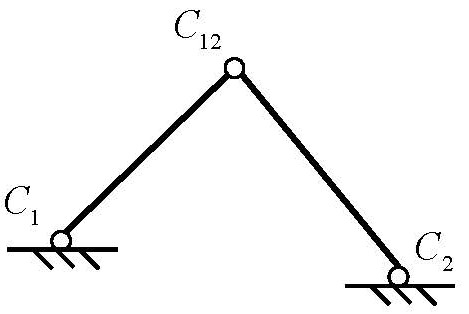
\includegraphics[width=0.2\linewidth]{immagini/1.PARTE4_Pagina_05}
\end{figure}

\[
\begin{cases}
	t=2 \\
	s=6 \Rightarrow 3t-s=0
\end{cases} 
\]
Notando poi che $ C_1, C_2, C_{12}$ sono palesemente NON allineati, allora $l = 0$ e quindi:

\[
\begin{split}
3t-s & = l - i \\
0 & = 0 - i
\end{split}  \Rightarrow i = 0 
\]
Tutti i vincoli sono necessari all'equilibrio: se elimino un vincolo introduco un grado di labilità, d'altro canto $l=0$ quindi non esistono spostamenti ammissibili con i vincoli. \newline 

\textbf{Esempio 2:} \newline 
\begin{figure}[H]
	\centering
	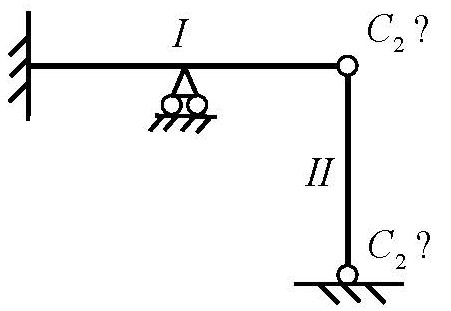
\includegraphics[width=0.2\linewidth]{immagini/1.PARTE4_Pagina_06 (1)}
\end{figure}
\[
\begin{cases}
	3t=6 \\
	s=8 
\end{cases} \Rightarrow 3t-s=-2
\]
Il corpo 1 è fermo a causa dell'incastro in A, è come se $C_2$ ora fosse un vincolo esterno, il corpo 2 non può che essere fermo: i due possibili centro di spostamento in B e C sono allineati, ma $C_2$ è contemporaneamente in due punti, e questo non può essere, si conclude così che $C_2 \nexists$ e la struttura è ferma $l =0$, allora:
\[
\begin{split}
	3t-s & = l - i \\
	-2 & = 0 - i \Rightarrow i = 2
\end{split}  
\]
Due vincoli possono essere rimossi senza intaccare teoricamente la labilità, ma che succede se si rimuove un vincolo essenziale e non sovrabbondante? Questo influenzerà la labilità? 

\newpage

\textbf{Esempio 3:} \newline 
\begin{figure}[H]
	\centering
	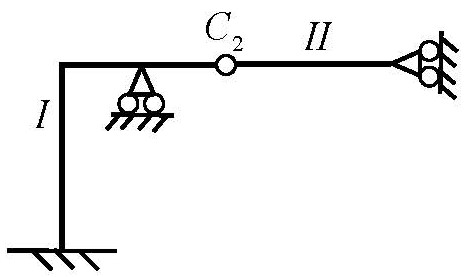
\includegraphics[width=0.2\linewidth]{immagini/1.PARTE4_Pagina_06}
\end{figure}
\[
\begin{cases}
	3t=6 \\
	s=7 
\end{cases} \Rightarrow 3t-s=-2
\]
Il corpo 1 è fermo a causa dell'incastro in A, il corpo 2 ha il suo centro di spostamento $C_2 \equiv C$ e dunque, potendo determinare univocamente il centro di spostamento $l=1$ e allora:
\[
\begin{split}
	3t-s & = l - i \\
	6-7 & = 1 - i \Rightarrow i = 2
\end{split}  
\]
Rimuovendo il vincolo che nell'esempio precedente era fornito dalla cerniera, questo raffigurato dal carrello, la labilità è stata modificata, quindi si, rimuovere un vincolo essenziale altera la labilità. \newline 

{\Large \textbf{Teorema degli Spostamenti Virtuali}} \mbox{} \newline
Entrano a questo punto in gioco i carichi esterni che a differenza di $l$ ed $i$ - queste caratteristiche della struttura - saranno in grado di dirci se un corpo è in equilibrio o meno. \newline

\newtheorem*{thm}{Teorema}

\begin{thm}
	Un corpo è in equilibrio se e solo se le forze esterne compiono lavoro virtuale nullo considerando i vincoli lisci e perfetti.
\end{thm} 

\[
L_V = \vec{f} \cdot \vec{s} = 0 ~~~~~ \forall \vec{s} \in \ker[C]
\]
Dove $ \vec{s} $ è un campo di spostamenti compatibile coi vincoli tale per cui $[C]\cdot s = 0$. \newline 

\newtheorem*{defn}{Spazio Ortogonale}

\begin{defn}
	Dato uno spazio V, si definisce spazio ortogonale lo spazio formato da tutti i vettori ortogonali agli elementi di V.
\end{defn} 

\[
\ker[A] = \left\lbrace Im[A]^T \right\rbrace^{\perp}  \leftrightarrow Im[A]^T =\left\lbrace \ker[A]\right\rbrace ^{\perp}
\]
\[
\ker[A]^T = \left\lbrace Im[A] \right\rbrace^{\perp}  \leftrightarrow Im[A] =\left\lbrace \ker[A]^T\right\rbrace ^{\perp}
\]

\begin{proof}
	Ricordando che \([E]\cdot\vec{\lambda} = \vec{f}\):
	\[
	\begin{cases}
		\vec{f} \in ~ Im[E] \\
		Im[E] = [\ker[E]^T]^{\perp}
	\end{cases} \Rightarrow Im[E] = [\ker[C]]^{\perp}
	\]
	In caso di vincoli perfetti:
	\[\vec{\delta} = 0 \Rightarrow [C]\cdot \vec{s} = 0 \Rightarrow \vec{s}\in \ker[C]\]
	
	\[
	L_V = \vec{f} \cdot \vec{s} \Rightarrow \begin{cases}
		\vec{f} \in [\ker[C]]^{\perp}\\
		\vec{s} \in \ker[C]
	\end{cases} \Rightarrow \vec{f} \perp \vec{s} \Rightarrow L_V = 0 \]

 
Se $l =0$ vale l'equilibrio per ogni forza applicata, qualsiasi sistema di forze applicato soddisfa l'equilibrio in quanto l'unico spostamento compatibile è quello nullo: 

\[ L_V = \vec{f} \cdot \vec{s} ~~~~ \forall \vec{f} \]
 
 Se $l \ne 0 \Rightarrow \exists \infty^l$ spostamenti ammissibili per cui si ha equilibrio se e solo se è rispettato il teorema degli spostamenti virtuali: sono sempre in grado di trovare un set di equazioni vincolari compatibili in cui per trovare l'equilibrio impongo il teorema degli spostamenti virtuali. \newline 
\end{proof}
 
 La labilità fornisce informazioni sull'esistenza delle soluzioni del problema di equilibrio, del problema della statica. \newline
 
 Ricapitolando: 
 \begin{itemize}
 	\item[$ i $] dà informazioni sul numero di soluzioni di equilibrio; 
 	\item[$ l $] dà informazioni sull'esistenza delle soluzioni di equilibrio:
 	\begin{description}
 		\item[$l = 0$] le soluzioni esistono;
 		\item[$l\ne0$] le soluzioni esistono solo se $\vec{f} \cdot \vec{s} = 0$;
 	\end{description}
 \end{itemize} 

	\textbf{Esempio} 
	\begin{figure}[H]
		\centering
		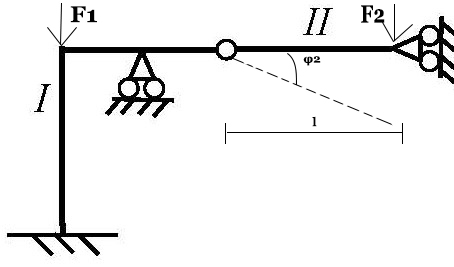
\includegraphics[width=0.4\linewidth]{immagini/1.PARTE4_Pagina_09}
	\end{figure}
	Nell'esempio qui riportato si era visto come $l=1, i=2$. 
	
	Come si comporta la struttura ora con forze applicate? \newline 
	
	Devo applicare il teorema degli spostamenti virtuali. 
	\[ \vec{F}\cdot\vec{s}=0\]
	
	$\vec{F_1} \cdot \vec{s} = 0$ allora dato che il punto d'angolo non si sposta, esiste un sistema di forze equilibrabile.
	
	Inoltre si può considerare equivalentemente il caso in cui $F_1$ sia applicata alla cerniera. Che spostamenti ammette quel punto sul corpo? Ricordando le condizioni sulla cerniera, si conclude che essendo $\vec{s} = 0$, il teorema degli spostamenti virtuali è verificato. \newline
	
	$\vec{F_2} \cdot \vec{s} =F_2\varphi_2l\ne 0$, questa è una forza che non possono contrastare con la reazioni vincolare applicata dal quel vincolo, non esiste alcuna reazione vincolare in grado di contrastarla, la forza non è equilibrabile. \newline 

 \newpage

  {\Large \textbf{Teorema delle Forze Virtuali}} \mbox{} \newline
  
  \begin{thm}
  	Il problema della compatibilità ha soluzione se e solo se il lavoro virtuale che le reazioni vincolari autoequilibrate compiono per la presenza di cedimenti è nullo.
  \end{thm}

  \[
  L_V = \vec{\lambda} \cdot \vec{\delta} = 0 ~~~~~ \forall  \vec{\lambda} \in \ker[E]
  \]
  
  In altre parole $\vec{\lambda}$ è il campo di reazioni vincolari autoequilibrate, ovvero tutte quelle reazioni vincolari che si hanno in presenza di carichi esterni nulli:
  
  \[
  \vec{f} = 0 \rightarrow [E] \cdot \vec{\lambda} = 0
  \]
  \begin{proof}
  	\[
  	\begin{cases}
  		\vec{\delta} \in Im[C] \\
  		Im[C] = [\ker[C]^T]^{\perp} \\
  		[C]^T = [E]
  	\end{cases} \Rightarrow Im[C] = [\ker[E]]^{\perp}
  	\]
  	\[
  	L_V = \vec{\lambda} \cdot \vec{\delta} = 0 \Rightarrow \begin{cases}
  		\vec{\delta} \in [\ker[E]]^{\perp} \\ 
  		\vec{\lambda} \in \ker{E}
  	\end{cases} \Rightarrow \vec{\delta} \perp \vec{\lambda} \Rightarrow L_V = 0
  	\]
  \end{proof} 
  
 Applicando il teorema delle forze virtuali all'esempio precedente rimasto irrisolto si ottiene che, considerando i due corpi separatamente: 
  \begin{figure}[H]
 	\centering
 	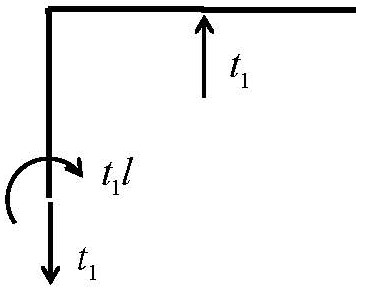
\includegraphics[width=0.25\linewidth]{immagini/1.PARTE4_Pagina_11 (2)}
 \end{figure}
  Scelgo un sistema di forze autoequilibrato: posso utilizzare come parametro per trovare le restanti reazioni la reazione $t_1$ del carrello. \newline
 
 L'unico vincolo che può equilibrare la reazione del carrello è l'incastro che compensa anche il momento. \newline
 \begin{figure}[H]
 	\centering
 	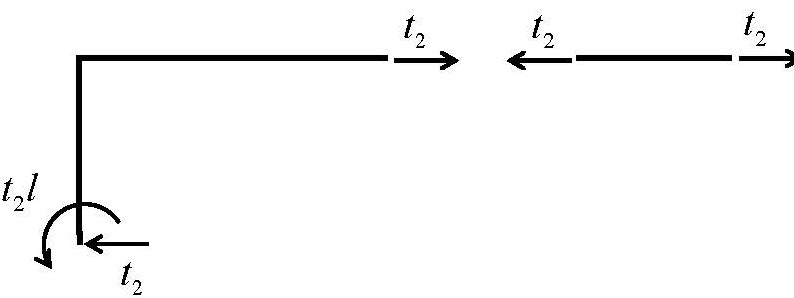
\includegraphics[width=0.35\linewidth]{immagini/1.PARTE4_Pagina_11}
 \end{figure}
 Utilizzo poi la reazione $t_2$ del carrello del secondo corpo.
 L'equilibrio del secondo corpo è garantito dalla cerniera interna, equilibrata dall'incastro.
 
 \newpage
 
 E se fossero presenti cedimenti? Quelli in figura sono compatibili? 
 \begin{figure}[H]
	\centering
	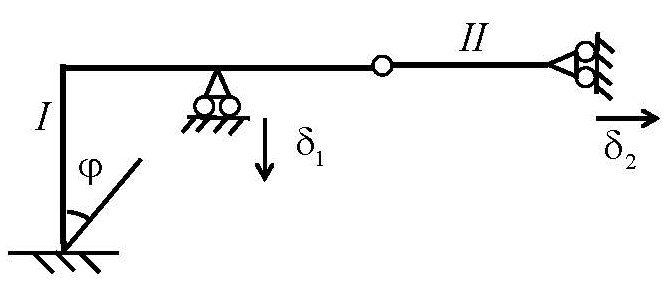
\includegraphics[width=0.35\linewidth]{immagini/1.PARTE4_Pagina_12 (2)}
\end{figure}
 In una struttura di questo tipo non è detto che i cedimenti siano compatibili, bisogna ricorrere al teorema delle forze virtuali. 
 \[
 \vec{\lambda} \cdot \delta = 0 \Leftrightarrow \begin{cases}
 	-t_1 \delta_1 + t_1 l \varphi = 0 & \Rightarrow \delta_1 = \varphi l ~~~~~ \forall t_1 \\
 	t_2 \delta_2 - t_2 l \varphi = 0 & \Rightarrow \delta_2 = \varphi l ~~~~~ \forall t_2
 \end{cases}
 \]
 
 Se avessimo avuto $ i = 0 \Rightarrow i = \dim[\ker{[E]}] \Rightarrow \ker{[E]} \Def 0 \Rightarrow \vec{\lambda} \cdot \vec{s} = 0 ~~~~~ \forall \vec{\delta}$
 
 Sempre nullo, non ho possibilità di autoequilibrio delle reazioni vincolari. 
 
 Una struttura \textbf{NON} iperstatica è sempre compatibile con i cedimenti.\newline
 
 Se $ i > 0$ e cioè la struttura è iperstatica, non è detto che qualsiasi cedimento sia compatibile, bisogna perciò ricorrere al teorema delle forze virtuali. \newline
 
 \textbf{L'iperstaticità fornisce informazioni dell'esistenza delle soluzione del problema della compatibilità, del problema della cinematica.}  \newline 
 
 Nella seguente tabella il primo caso che si analizza è quello del problema statico per struttura iperstatica, ad essendo $i=0$ esiste una sola soluzione di equilibrio, mentre per $l=0$ esisterà equilibrio $\forall\vec{f}$.
 
 Viceversa sarà per la compatibilità degli spostamenti.
 
\begin{figure}[H]
	\centering
	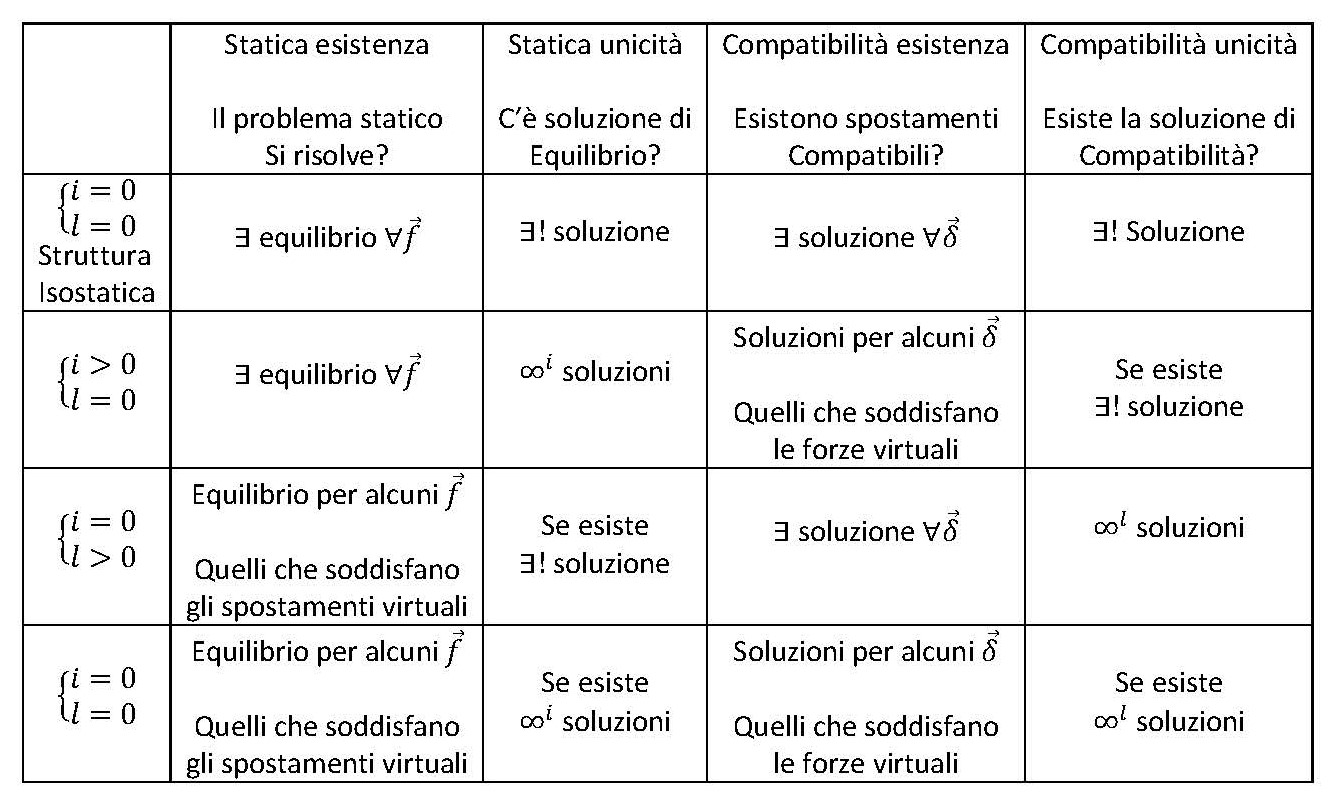
\includegraphics[width=0.8\linewidth]{immagini/tab}
\end{figure}

\begin{itemize}
	\item $ \begin{cases}
		i \geq 0 \\
		l \geq 0
	\end{cases}$ perché sono dimensioni di spazi vettoriali;
\item $ 3t-s>0 \Rightarrow l>0$ significa che esistono obbligatoriamente i centri di spostamento compatibili: $s<3t$;
\item   $ 3t-s<0 \Rightarrow i>0$, ci sono vincoli superflui: $s>3t$;
\item   $ 3t-s=0 \Rightarrow l=i$ ma non è detto che la struttura sia isostatica.
\end{itemize}

\newpage

\textbf{{\Large Applicazione} }
\begin{figure}[H]
	\centering
	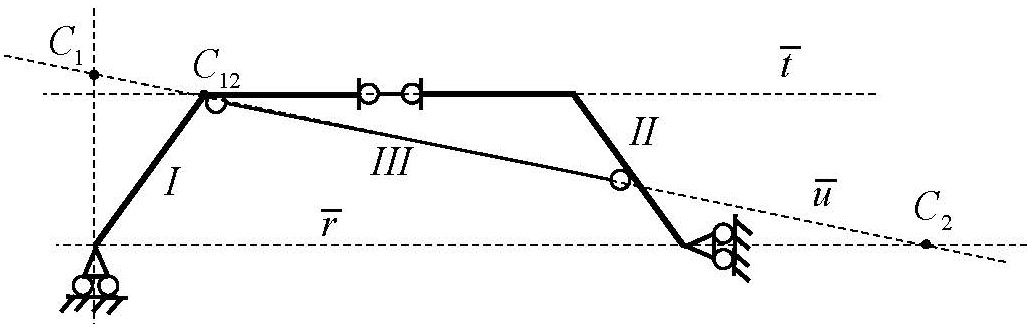
\includegraphics[width=0.55\linewidth]{immagini/1.PARTE4_Pagina_14}
\end{figure}
Il terzo corpo, non essendo
direttamente caricato ed
avendo le stesse restrizioni
cinematiche di un pendolo, può
essere considerato un pendolo.

Perciò se il corpo 3 è un pendolo ottengo: 
\[
\begin{cases}
	t = 2\\
	s = 4
\end{cases} \Rightarrow 3t - s = 2 > 0 \Rightarrow \text{sicuramente esistono i centro di spostamento}
\]

Siccome il centro relativo è fissato, mi basta scegliere la posizione di un centro assoluto per trovare immediatamente l'altro centro assoluto attraverso l'allineamento e dunque $g = 1 \Rightarrow l = g+ 1 = 2$: 
\[
\begin{split}
	3t - s & = l-1 \\
	2 & = 2-i \Rightarrow i = 0
	\end{split}
\]
Da notare come per il corpo 2, lo spostamento assoluto dei centri di spostamento sia identico: il punto \textcolor{red}{\textbf{X}} è caratterizzato relativo da spostamento non nullo ma spostamento assoluto identico a causa di $C_{12}$.
\begin{figure}[H]
	\centering
	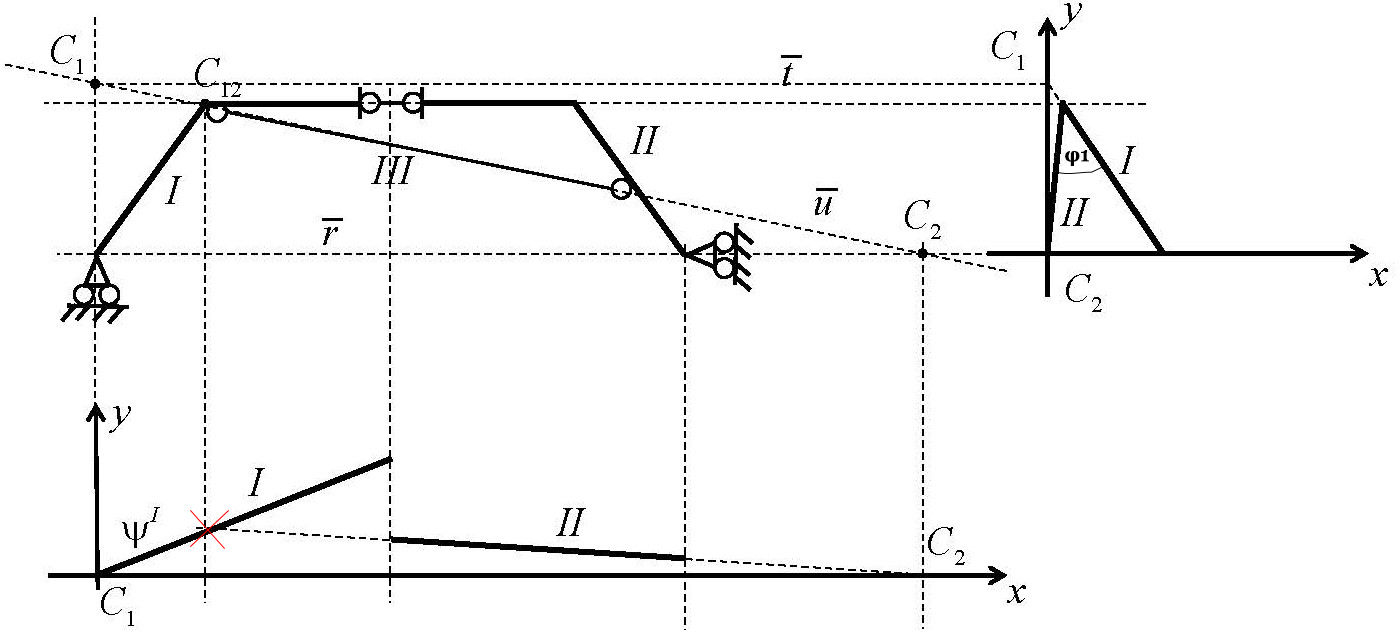
\includegraphics[width=0.5\linewidth]{immagini/1.PARTE4_Pagina_15}
\end{figure}

	E se avessimo avuto $C_2\rightarrow\infty$ improprio? 

\begin{figure}[H]
	\centering
	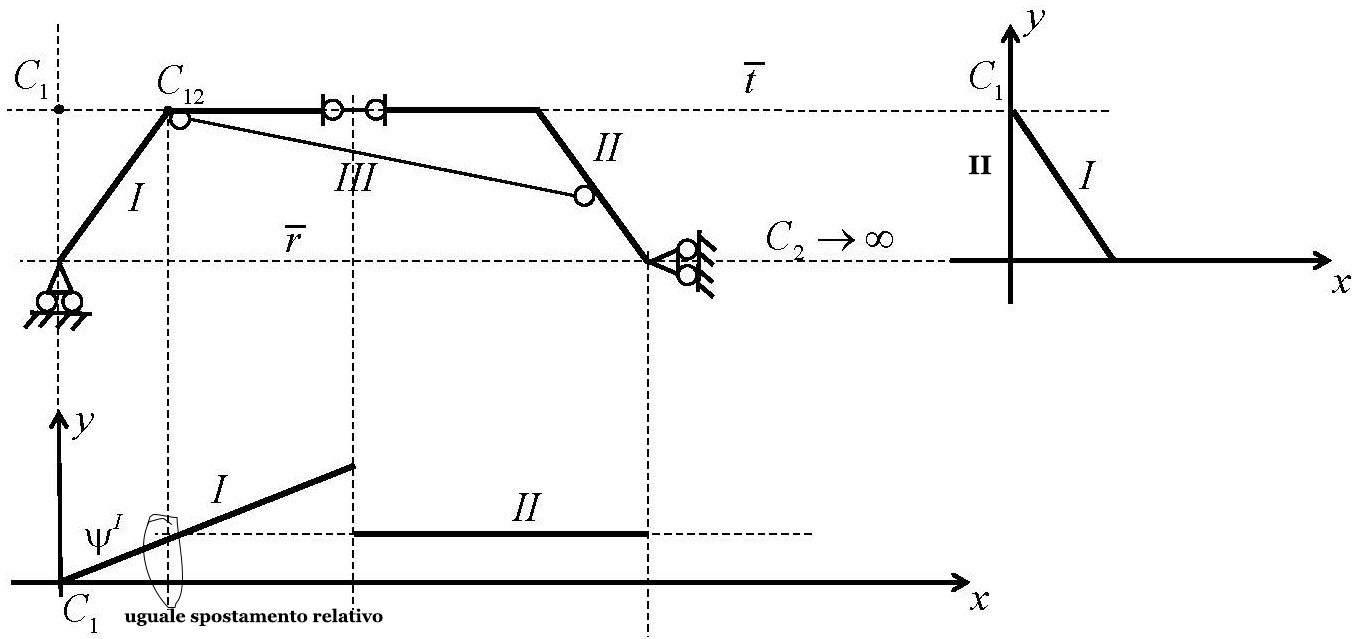
\includegraphics[width=0.5\linewidth]{immagini/1.PARTE4_Pagina_16}
\end{figure}

	Ricorda che un punto improprio non è caratterizzato da rotazione ma da traslazione nella direzione ortogonale rispetto alla quale sta il centro di spostamento, è per questo che $s''_x = 0$.
	
	Nota inoltre come il punto cerchiato sia sempre caratterizzato da spostamento relativo nullo e spostamento assoluto non nullo, sempre a causa di $C_{12}$.\newline 

{\Large \textbf{Metodo di Lagrange}} \mbox{} \newline
Si tratta di un metodo per trovare la reazione vincolare di un \underline{singolo vincolo} all'interno di una struttura, per fare una specifica verifica, magari.

Sfruttando il fatto che ogni vincolo
multiplo può essere rappresentato come una somma di vincoli semplici. \newline

Si definisce
vincolo essenziale un vincolo semplice che viene rappresentato da una riga indipendente
della matrice C: eliminando una riga varierà per forza $\rk[C]$ variando conseguentemente anche $l$.

Quando un vincolo è essenziale, se viene eliminato varia il rango della matrice C, per cui varia la labilità
della struttura. \newline

Nell'esempio seguente i vincoli sono entrambi essenziali perché danno restrizioni
differenti.
Rimuovendone uno la labilità passerebbe da 1 a 2.
\begin{figure}[H]
	\centering
	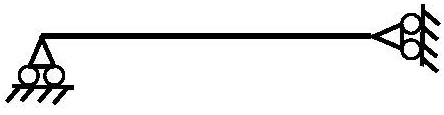
\includegraphics[width=0.15\linewidth]{immagini/1.PARTE4_Pagina_17}
\end{figure}

Si definisce
vincolo sovrabbondante un vincolo semplice che può essere rappresentato da una riga
dipendente nella matrice C: un vincolo che se rimosso non apporta variazione a $\rk[C]$ e dunque alla labilità $l$.\newline

Un vincolo sovrabbondante dà una restrizione cinematica che viene già fornita da un altro vincolo, per
cui se viene eliminato non varia né il rango di C, né e la labilità della struttura né varia la
possibilità di spostamento della struttura. \newline

Perciò a partire da una struttura in equilibrio per conoscere la reazione di un singolo vincolo che sia semplice
ed essenziale bisogna eliminare il vincolo e sostituirlo con una generica reazione vincolare che questo
può esercitare, e in seguito applicare il principio degli spostamenti virtuali.

Nella pratica per verificare l'essenzialità di un vincolo lo si toglie e si verifica se cambia $l$ ricalcolando i centro di spostamento. \newline

\textbf{Struttura appoggio - appoggio}
\begin{figure}[H]
	\centering
	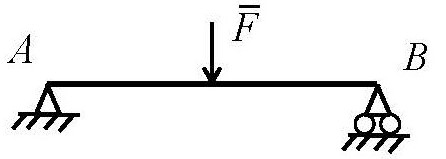
\includegraphics[width=0.25\linewidth]{immagini/1.PARTE4_Pagina_18 (2)}
\end{figure}
\[
\begin{split}
	3t - s = 0 & \Rightarrow l - i = 0 \Rightarrow l = i \\
	l =0 & \Rightarrow i = 0 \rightarrow ~ \text{La struttura è isostatica}
\end{split}
\]
Non riesco ad identificare alcun centro $C$.\newline

 Se voglio trovare la reazione vincolare in B, sostituisco il carrello con una forza vincolare. 
 \begin{figure}[H]
 	\centering
 	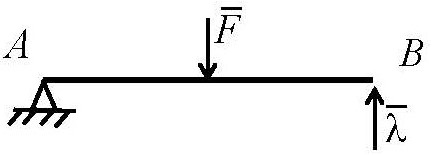
\includegraphics[width=0.25\linewidth]{immagini/1.PARTE4_Pagina_18 (3)}
 \end{figure}
 Poiché la struttura è in equilibrio applico il principio degli spostamenti virtuali agli spostamenti compatibili. 
 \begin{figure}[H]
	\centering
	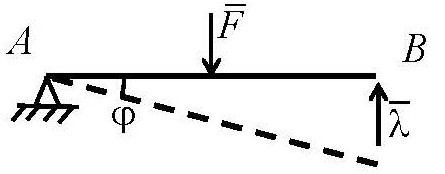
\includegraphics[width=0.25\linewidth]{immagini/1.PARTE4_Pagina_18}
\end{figure}
 \[
 L_V = F\varphi \frac{l}{2} - \lambda \varphi l = 0 \Rightarrow \lambda = \frac{F}{2}
 \] 
 
 \[
 R= \lambda = \frac{F}{2}
 \]
 
 \textbf{Esempio 1}
 \begin{figure}[H]
	\centering
	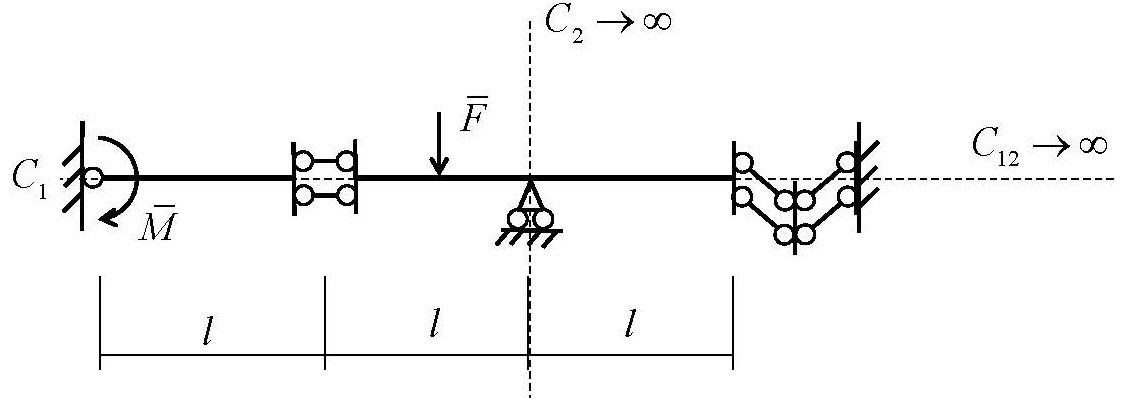
\includegraphics[width=0.65\linewidth]{immagini/1.PARTE4_Pagina_19 (2)}
\end{figure}
 I 3 centri di spostamento non sono allineati, essendoci due punti impropri, questi non appartengono a rette parallele $\Rightarrow l = 0 \Rightarrow  \newline 3t-s = 6-6 = 0 = l - i \Rightarrow 0 = 0 - i \Rightarrow i = 0$ \newline e tutti i vincoli sono essenziali. \newline 
 
Da questo esempio si ricavi la reazione del doppio doppio pendolo.

Applicando Lagrange si sostituisce la reazione vincolare del doppio pendolo (il momento angolare $\vec{\lambda}$) al posto del vincolo e si applica il principio degli spostamenti virtuali. 
 \begin{figure}[H]
	\centering
	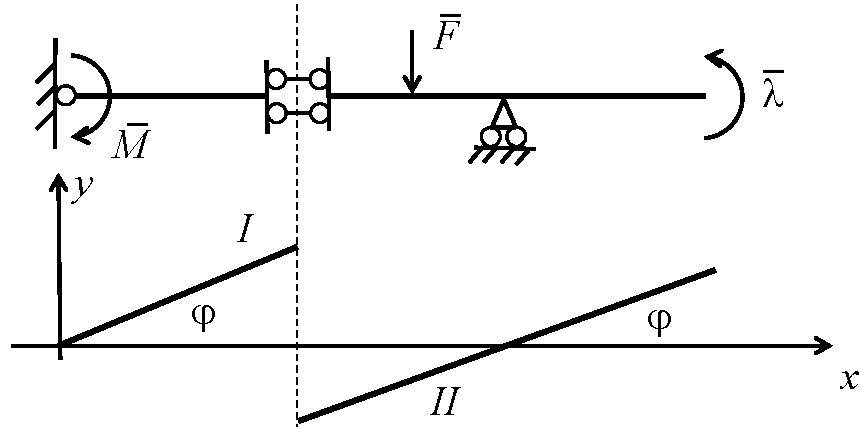
\includegraphics[width=0.4\linewidth]{immagini/1.PARTE4_Pagina_19}
\end{figure} 
Notare sempre come il doppio pendolo interno imponga rotazioni uguali.
 \[
 L_V = -M \varphi + F\varphi \frac{l}{2} + \lambda \varphi = 0
 \]
 \[
 \lambda = M - F\frac{l}{2}
 \]
 Se la struttura non fosse stata iperstatica si doveva dimostrare che la struttura era in equilibrio, applicando gli spostamenti virtuali, e dimostrare che quello specifico vincolo era essenziale. \newline \newpage
 
 \textbf{Esempio 2} \newline 
 Si voglia trovare $\mu$ tale che la struttura risulti in equilibrio: risolvere in forma parametrica dimostrando l'equilibrio della struttura. \newline 
 
  \begin{figure}[H]
 	\centering
 	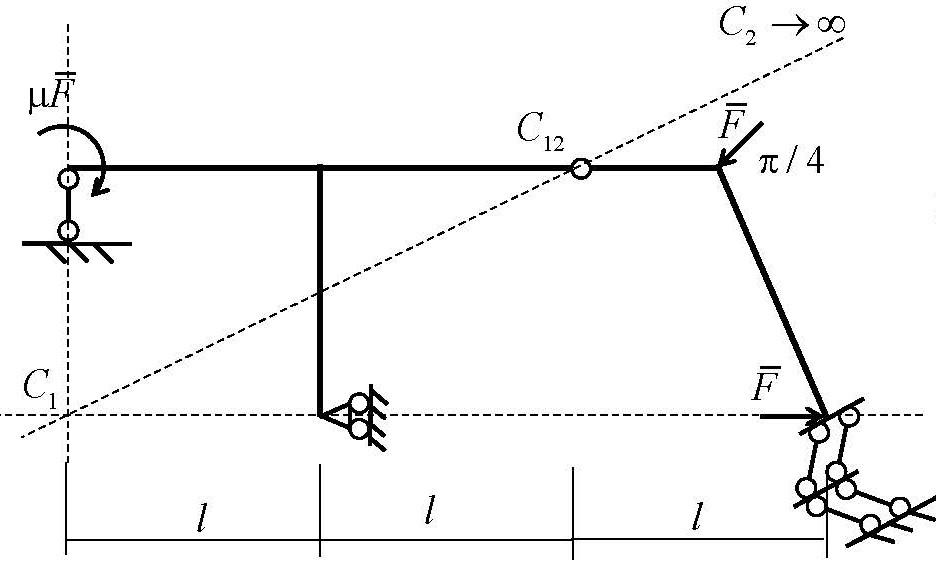
\includegraphics[width=0.4\linewidth]{immagini/1.PARTE4_Pagina_20}
 \end{figure}
 
 Poiché due punti propri definiscono una direzione, per l'allineamento $C_2$ si troverà all'infinito lungo quella direzione, essendo stati i centri di spostamento determinati senza incertezze:
 \[ g = 0 \hspace{1cm} l = 1 \hspace{1cm} 3t - s = l - i \Rightarrow 5-6 = 1-i \Rightarrow i = 0\]
 Tutti i vincoli sono essenziali. \newline 
 
 Essendo $i = 0; l>0$ esiste equilibrio solo per alcuni $\vec{f}$ ottenuti applicando gli spostamenti virtuali: 
 \[L_v = \vec{f}\cdot\vec{s} = 0\]
 
 \begin{figure}[H]
 	\centering
 	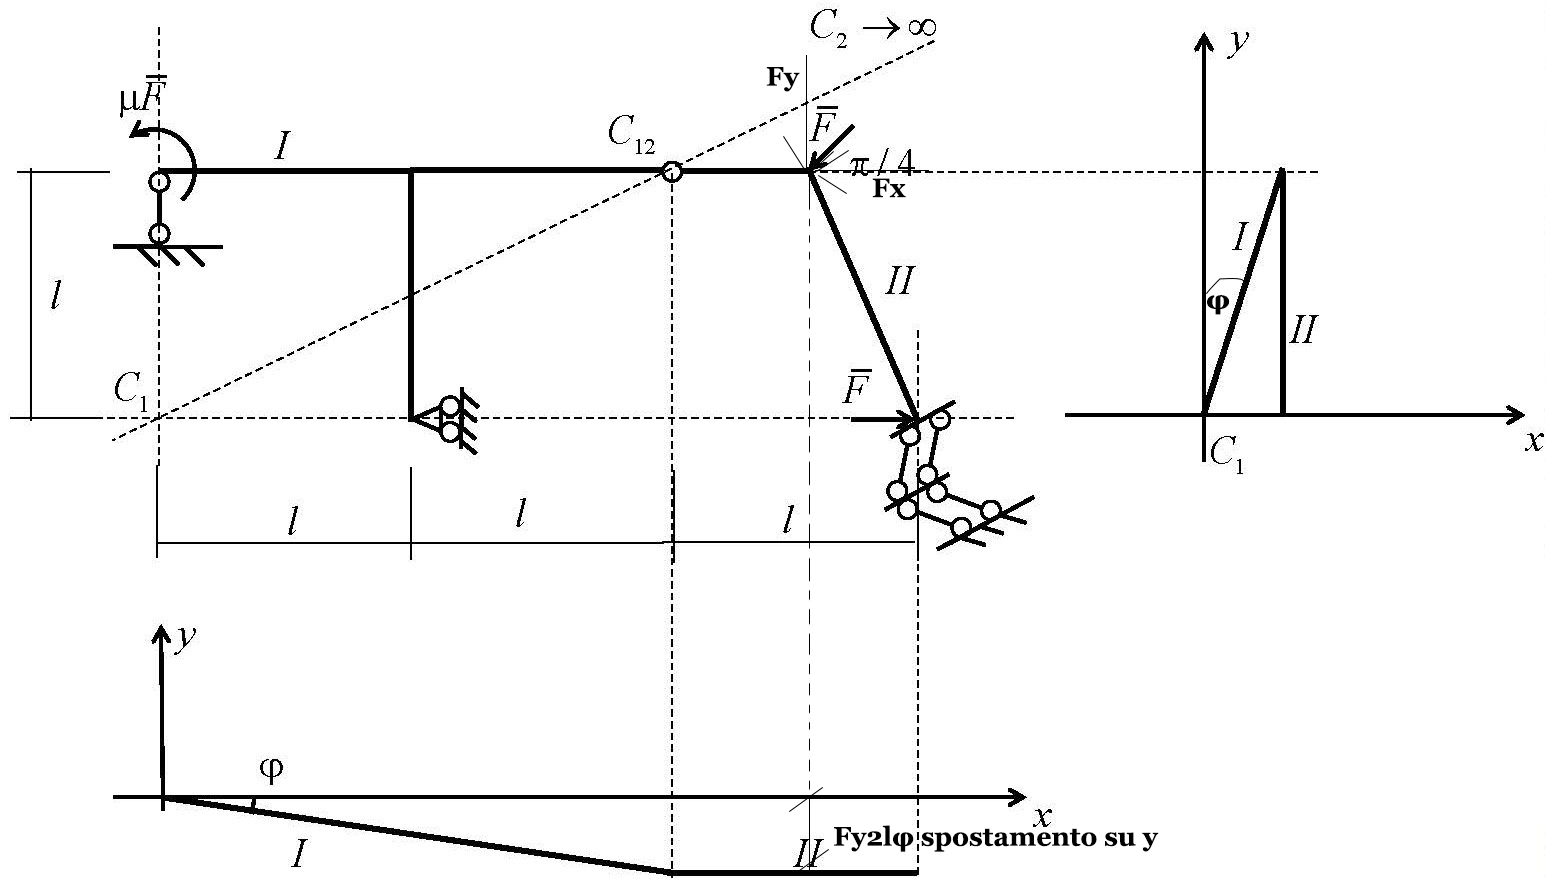
\includegraphics[width=0.5\linewidth]{immagini/1.PARTE4_Pagina_21}
 \end{figure}
 
 \begin{eqnarray*} L_V = -\mu F\varphi - {\sqrt{2}\over2}F\varphi l + {\sqrt{2}\over2}F\varphi 2l + F\varphi l = 0 \\
 \mu = \dfrac{2+\sqrt{2}}{2}l 
\end{eqnarray*}

Avendo dimostrato il sistema essere in equilibrio, posso applicare Lagrange per trovare la reazione verticale della cerniera intera. 
\newpage
Questa, ora divenuta pendolo, rende il centro di spostamento relativo $C_{12}$ punto proprio sulla retta $r$, scelto ad arbitrio per essere allineato a $C_1$, con $C_2\rightarrow\infty$: restringendo il campo di possibilità si sceglie dove porre  $C_{12}: g = 1$. 

\begin{figure}[H]
	\centering
	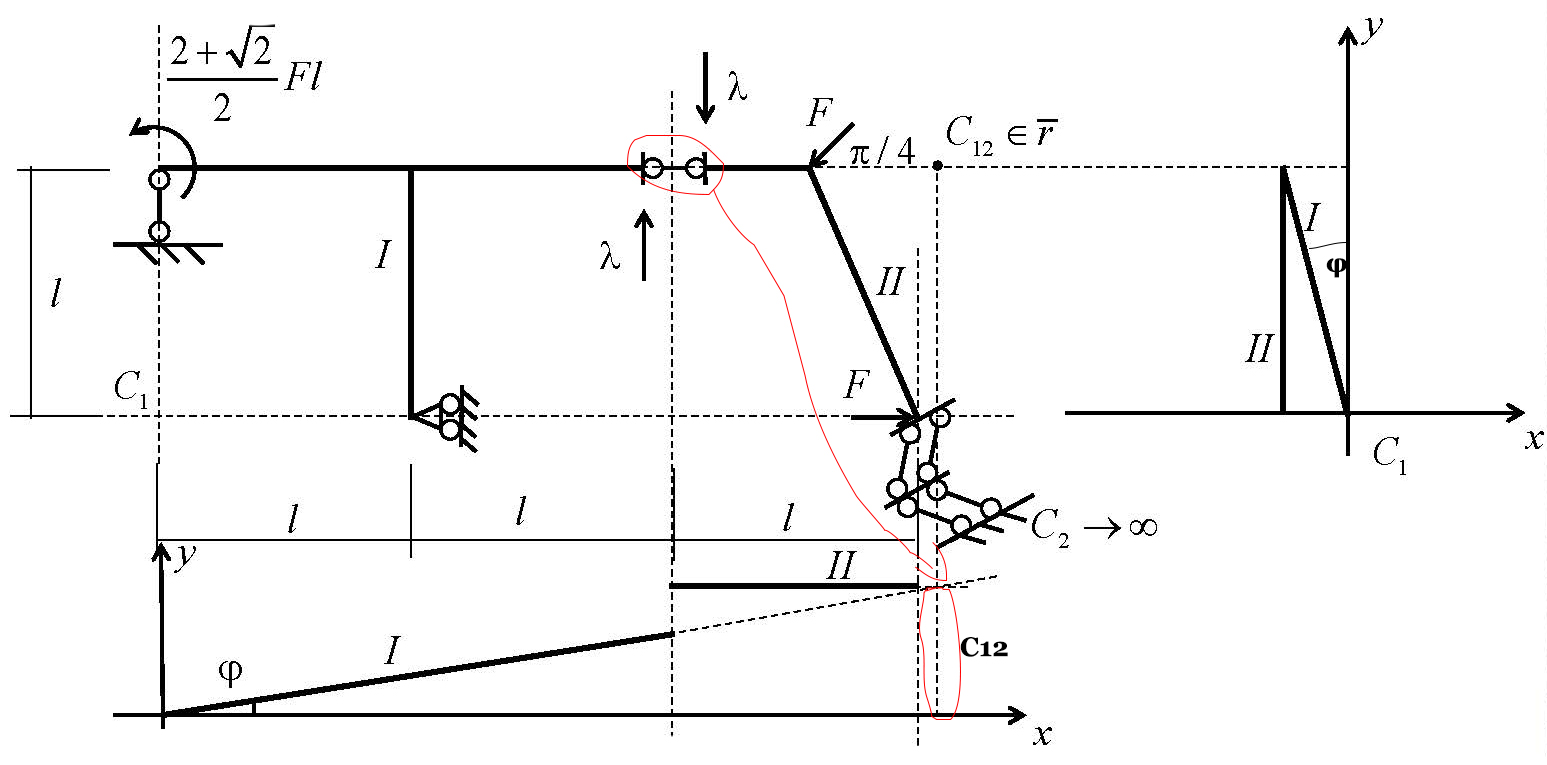
\includegraphics[width=0.5\linewidth]{immagini/1.PARTE4_Pagina_22}
\end{figure}

\[ g = 1  \hspace{1cm} l = 2 \hspace{1cm} 3t - s = l - i \Rightarrow 6-4 = 2-i \Rightarrow i = 0\]
\[ L_V = \dfrac{2+\sqrt{2}}{2}l  F\varphi l + \lambda\varphi2l - \lambda\varphi xl + {\sqrt{2}\over2}F\varphi l - {\sqrt{2}\over2}F\varphi xl - F\varphi l = 0 \]
\[\lambda = -{\sqrt{2}\over2} \]
Dove $x$ è la distanza alla quale si trova $C_{12}$, scelta arbitrariamente. \newline 

E se si cambiasse scelta di $C_{12}$? Lo si scelga anch'esso improprio come $C_2$, dalla teoria è noto che due punti impropri sono coincidenti all'infinito da questo, essendo:
\[C_2 = C_{12} \ne C_1\]
Dalla seconda proprietà dei centri di spostamento, il corpo 1 è fermo. 

\begin{figure}[H]
	\centering
	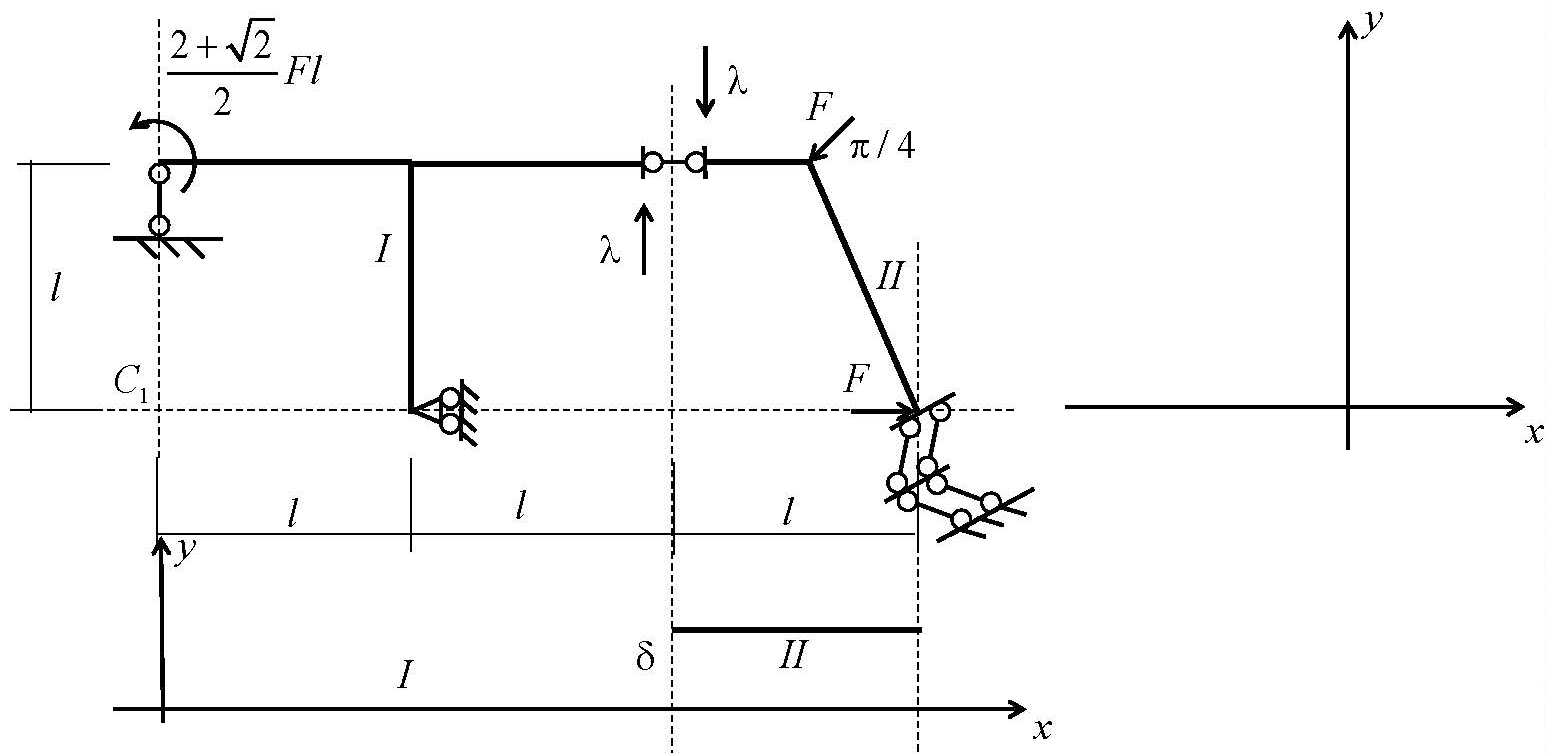
\includegraphics[width=0.5\linewidth]{immagini/1.PARTE4_Pagina_23}
\end{figure}

\[L_V = -\lambda\delta + {\sqrt{2}\over2}F\delta = 0 \Rightarrow \lambda = -{\sqrt{2}\over2}F \]
Con $\delta$ scelta arbitraria di traslazione.\newline \newpage
 
 {\Large \textbf{Metodo Grafico per le Reazioni Vincolari}} \mbox{} \newline
  \textbf{{\small VALIDO SOLO PER STRUTTURE A IPERSTATICITÀ NULLA $i =0$}} per cui è noto che esiste ed è unica la soluzione per ogni carico applicato. \newline 

\textbf{Trave appoggio - appoggio } \newline
Si era trovato che era una struttura ad iperstaticità nulla e dunque isostatica con $i=l$. 
\begin{figure}[H]
	\centering
	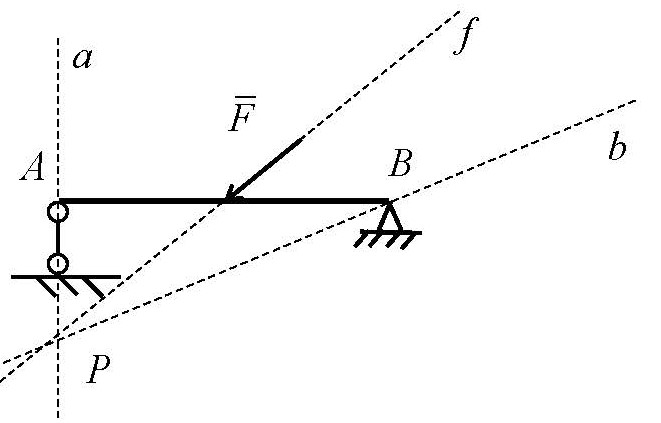
\includegraphics[width=0.4\linewidth]{immagini/1.PARTE4_Pagina_24}
\end{figure}

In questo caso si nota che la reazione del pendolo è parallela all'asse dello stesso ed è passante per A e la reazione della cerniera giace su una qualsiasi retta passante per B. 

Siccome tre forze per essere in equilibrio devono concorrere in uno stesso punto, la retta \underline{b} passerà dovrà incontrarsi dove si incontrano \underline{a} ed \underline{f}, per cui, l'equilibrio simbolico è dato da: 

\[
\underline{a} + \underline{b} + \underline{f} = 0 
\]
I moduli delle forze sono così tali da formare dei triangoli chiusi composti da vettori che si rincorrono.\newline 

Una struttura labile ha o non ha una soluzione di equilibrio in dipendenza dai carichi esterni. \newline

Per facilitare la visualizzazione del poligono chiuso traslo \underline{a} in modo da chiudere in maniera arbitraria il triangolo, d'altro canto ciò che si conosce è su che retta agisce A e la direzione di F, il poligono si chiuderà con vettori che si devono rincorrere, in questo modo si sono trovati i verso delle reazioni vincolari ignote. 
\begin{figure}[H]
	\centering
	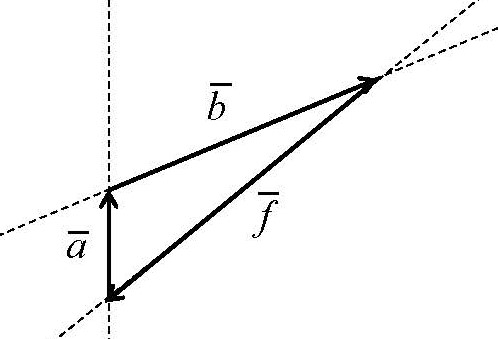
\includegraphics[width=0.4\linewidth]{immagini/1.PARTE4_Pagina_25 (2)}
\end{figure}
\newpage
\textbf{Trave appoggio - appoggio con momento concentrato}\newline
A differenza dell'applicazione di una forza concentrata, il grafico di un momento concentrato è ancor più qualitativo. 
\begin{figure}[H]
	\centering
	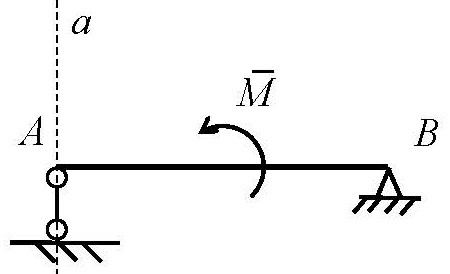
\includegraphics[width=0.4\linewidth]{immagini/1.PARTE4_Pagina_25 (3)}
\end{figure}
La reazione del pendolo è parallela all'asse dello stesso e passa per A.

Per rispettare l'equilibrio la reazione della cerniera in B dovrà essere parallela ad A, passante per B ed opposta a quella di A, con le direzioni relative date da M.

Quello che si deve rispettare è l'equilibrio a rotazione: un momento concentrato antiorario (+) genera una coppia di forze oraria, antioraria se M è orario.  \newline
\begin{figure}[H]
	\centering
	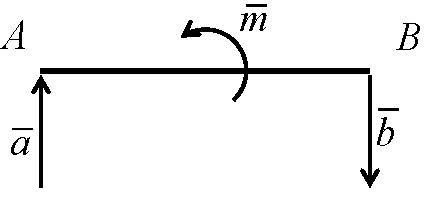
\includegraphics[width=0.4\linewidth]{immagini/1.PARTE4_Pagina_25}
\end{figure}
\newpage
\textbf{Esempio 1}
\begin{figure}[H]
	\centering
	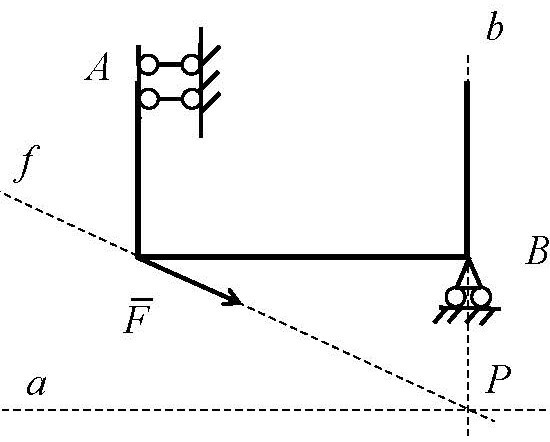
\includegraphics[width=0.4\linewidth]{immagini/1.PARTE4_Pagina_26 (2)}
\end{figure}
\[
3t - s = 3-3 = 0; i=l=0  ~ \text{e la struttura è isostatica}
\]
Il vincolo in A contribuisce sia con una forza che con un momento, che per quanto ci riguarda è possibile vedere come una forza traslata di un braccio $d$ la cui retta d'azione si può traslare dove serve. 

Alla fine bisognerà ricordarsi che in A agirà una reazione trovata graficamente PIÙ un momento pari a $\vec{m_a} = \vec{a} \cdot \bar{PA_y}$

\begin{figure}[H]
	\centering
	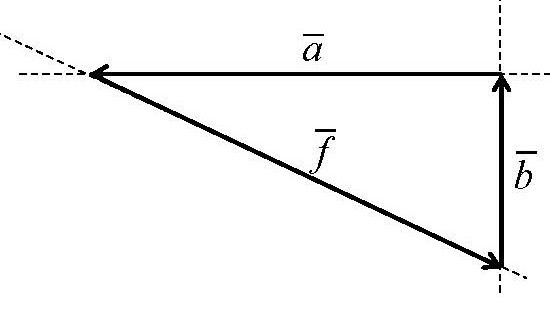
\includegraphics[width=0.15\linewidth]{immagini/1.PARTE4_Pagina_26}
\end{figure}

\textbf{Esempio 2.1: forza}
\begin{figure}[H]
	\centering
	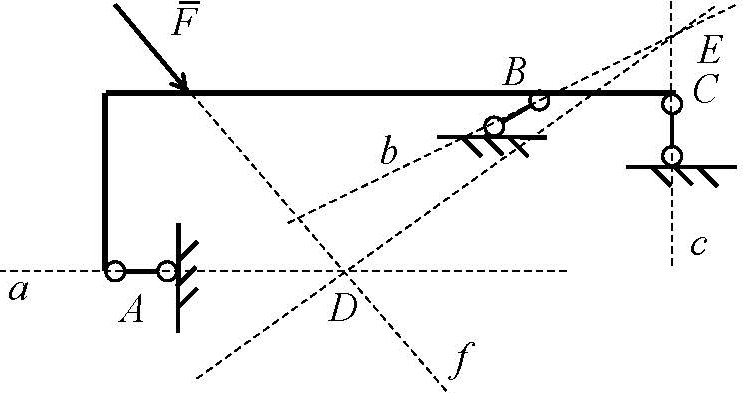
\includegraphics[width=0.4\linewidth]{immagini/1.PARTE4_Pagina_27 (2)}
\end{figure}
Le rette d’azione sono tutte fissate: \(CdS\in a,b,c \Rightarrow C\nexists \Rightarrow l = 0\) e posso applicare il metodo grafico: $l = i$.
\[
\underline{a} + \underline{b} + \underline{c} + \underline{f}= 0 
\]
Dal grafo della struttura si nota come sia comodo raggrupparle due a due in questo modo:
\[
(\underline{a} + \underline{f}) + (\underline{c} + \underline{b})= 0 
\]
Nella somma vettoriale di due vettori, questi si traslano in modo che l'origine di ognuno coincida con l'estremo del precedente. Il risultato si ottiene congiungendo l'origine del primo addendo con l'estremo dell'ultimo addendo. \newline

Si procede perciò calcolando la somma (\underline{a} + \underline{f}):
\begin{figure}[H]
	\centering
	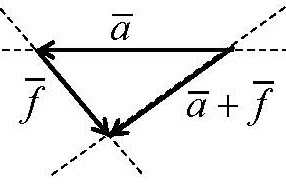
\includegraphics[width=0.15\linewidth]{immagini/1.PARTE4_Pagina_27 (3)}
\end{figure}
Ora che sono note 3 rette d'azione di tre vettori concorrenti in un punto (D), si può riscrivere un nuovo equilibrio per stabilire le direzioni dei vettori incogniti \newline \underline{c} + \underline{b}, ricordando prima di tutto che questi nuovi vettori dovranno concorrere in un nuovo punto in comune (E) e che in una somma di tre vettori, questi devono \textit{"rincorrersi"}.
\begin{figure}[H]
	\centering
	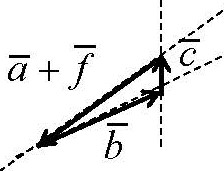
\includegraphics[width=0.15\linewidth]{immagini/1.PARTE4_Pagina_27 (4)}
\end{figure}
Stabilendo così la direzione di tutte le reazioni vincolari. 
\begin{figure}[H]
	\centering
	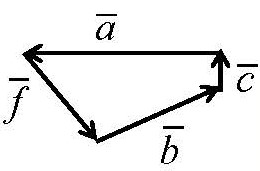
\includegraphics[width=0.15\linewidth]{immagini/1.PARTE4_Pagina_27}
\end{figure} 

\textbf{Esempio 2.2: momento} 
\begin{figure}[H]
	\centering
	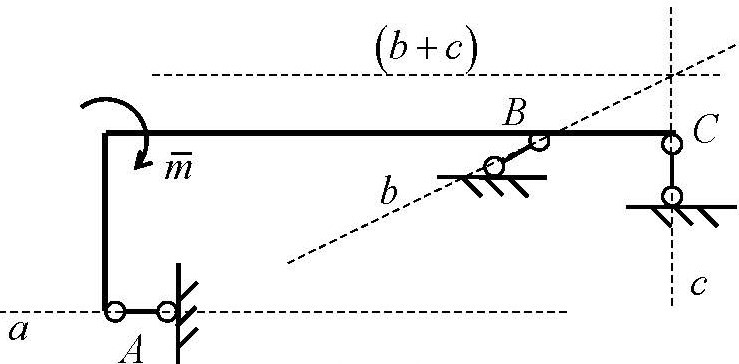
\includegraphics[width=0.4\linewidth]{immagini/1.PARTE4_Pagina_28 (3)}
\end{figure}
Le rette d’azione sono tutte determinate.
\[
\underline{a} + \underline{b} + \underline{c} + \underline{m}= 0 
\]
Dal grafo della struttura si nota come sia comodo raggrupparle in questo modo:
\[
\underline{a} + (\underline{b} + \underline{c}) + \underline{m}= 0 
\]
Si trova con una certa rapidità che la somma  (\underline{b} + \underline{c}) è una retta passante per l'intersezione di \underline{b} e \underline{c}.
\begin{figure}[H]
	\centering
	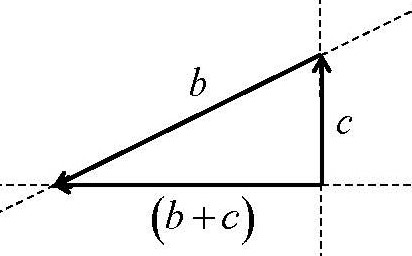
\includegraphics[width=0.15\linewidth]{immagini/1.PARTE4_Pagina_28 (2)}
\end{figure}

Tale retta è parallela alla retta \underline{a}, perciò conscio della presenza di un momento orario, su \underline{a} e (\underline{b} + \underline{c}) agirà una coppia di forze antioraria.
\begin{figure}[H]
	\centering
	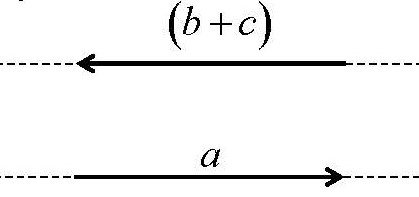
\includegraphics[width=0.15\linewidth]{immagini/1.PARTE4_Pagina_28 (4)}
		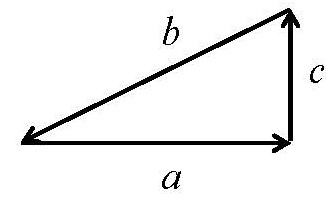
\includegraphics[width=0.15\linewidth]{immagini/1.PARTE4_Pagina_28}
\end{figure}

\begin{center}
	{\textbf{SE UNA STRUTTURA È IN EQUILIBRIO, OGNI SINGOLO CORPO SARÀ IN EQUILIBRIO}} 
\end{center}

\textbf{Esempio 3} \newline
E se lavoro con più corpi?

\begin{figure}[H]
	\centering
	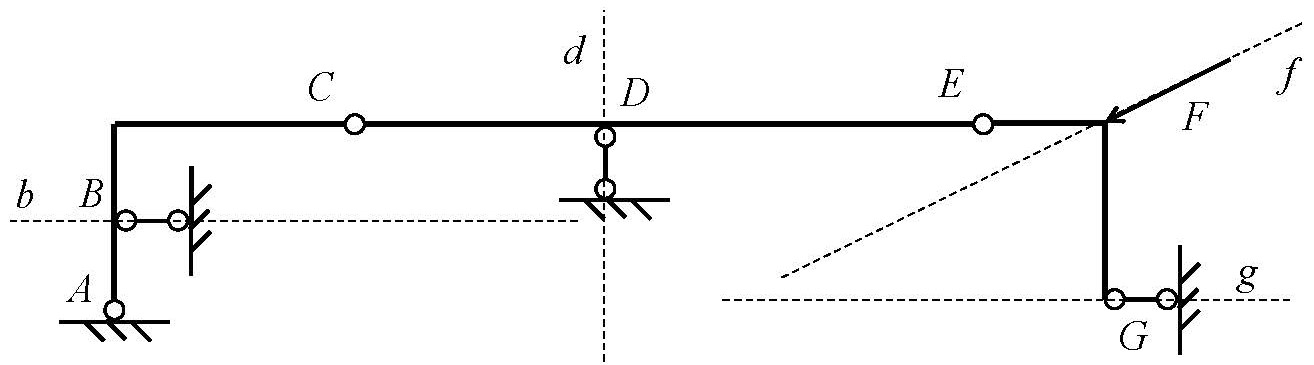
\includegraphics[width=0.5\linewidth]{immagini/1.PARTE4_Pagina_29}
\end{figure}
\[ 3t = 9 \Rightarrow 6 CdS;  s = 9 \Rightarrow 3t - s = 0\]
Il corpo 1 è fermo perché $C_1$ dovrebbe appartenere contemporaneamente ad $A$ e sulla retta \underline{b}. 

Il punto $C$ è ora equivalente ad una cerniera esterna, $C_2$ dovrebbe appartenere così a $C$ che alla retta \underline{d}.

Ugualmente per il corpo 3 IN $E$ la cerniera è divenuta esterna per cui $C_3$ dovrebbe appartenere sia ad $E$ che alla retta \underline{g}, anche il corpo 3 è fermo. 

La struttura è ferma. 
\[l=0\]
\[3t - s = l- i \Rightarrow 0 = 0 - i \Rightarrow l=i=0\]
La struttura è isostatica. \newline 

Si scrivano gli equilibri simbolici per ogni corpo:
\[\begin{aligned}
	1. & ~ \underline{a} + \underline{b} + \underline{c}'   = 0 \\
	2. & ~ \underline{c}'' + \underline{d} + \underline{e}''  = 0 \\
	3. & ~ \underline{e}''' + \underline{f} + \underline{g}  = 0 \\
\end{aligned}\]
L'equilibrio globale è la somma degli equilibri:
\[ \underline{a} + \underline{b} + \underline{c}' + \underline{c}'' + \underline{d} + \underline{e}'' + \underline{e}''' + \underline{f} + \underline{g} = 0 \]
Poiché:
\[ \begin{cases}
	\underline{c}' = -\underline{c}'' \\
	\underline{e}'' = -\underline{e}''' \end{cases} \]
\[ \underline{a} + \underline{b}  + \underline{d}  + \underline{f} + \underline{g} = 0 \]
Si è dimostrato come si può scrivere l'equilibrio globale come somma delle reazioni vincolari esterne e dei carichi esterni, vedendo la struttura come un corpo unico. 

\begin{figure}[H]
	\centering
	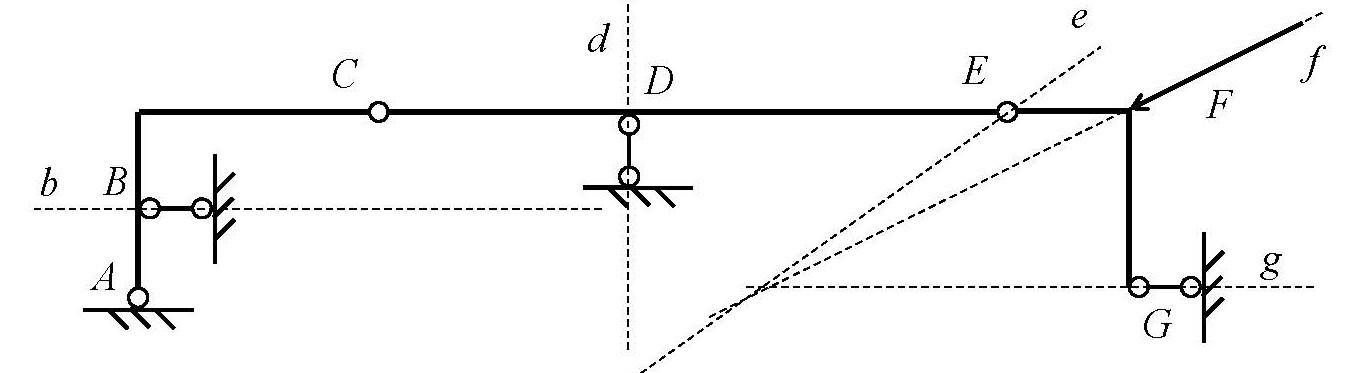
\includegraphics[width=0.5\linewidth]{immagini/1.PARTE4_Pagina_30.1}
\end{figure}

Dal terzo corpo è noto come tre rette debbano convergere in un unico punto, se la fanno già \underline{f}  e \underline{g}, allora \underline{e} non potrà fare altrimenti. 
\[\underline{e} + (\underline{f} + \underline{g}) = 0\]

\begin{figure}[H]
	\centering
	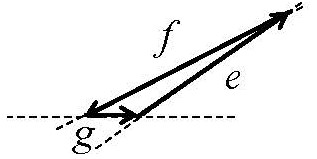
\includegraphics[width=0.15\linewidth]{immagini/1.PARTE4_Pagina_30}
\end{figure}

Ora che conosco la reazione di \underline{e} vado a ritroso sul corpo 2. 

\begin{figure}[H]
	\centering
	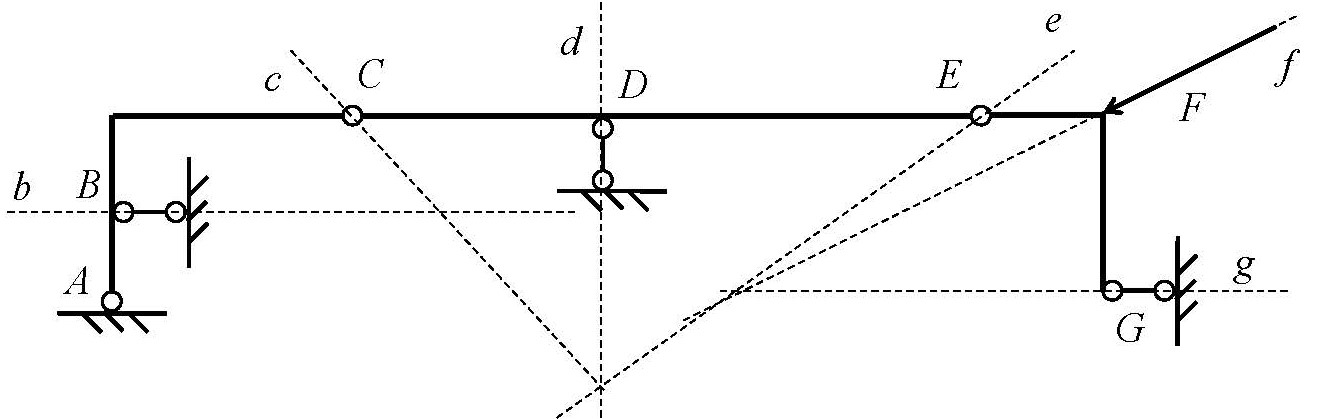
\includegraphics[width=0.5\linewidth]{immagini/1.PARTE4_Pagina_31.1}
\end{figure}

È la retta \underline{c} ora a dover passare nel punto d'intersezione tra \underline{d}  e \underline{e}:
\[\underline{c} + (\underline{d} + \underline{e}) = 0\]

\begin{figure}[H]
	\centering
	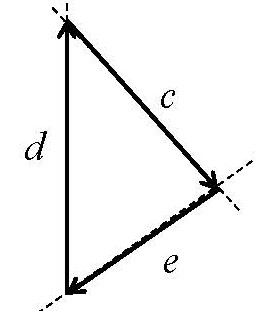
\includegraphics[width=0.15\linewidth]{immagini/1.PARTE4_Pagina_31}
\end{figure}

Ora che conosco la reazione in  \underline{c} posso passare al corpo 1. 

\begin{figure}[H]
	\centering
	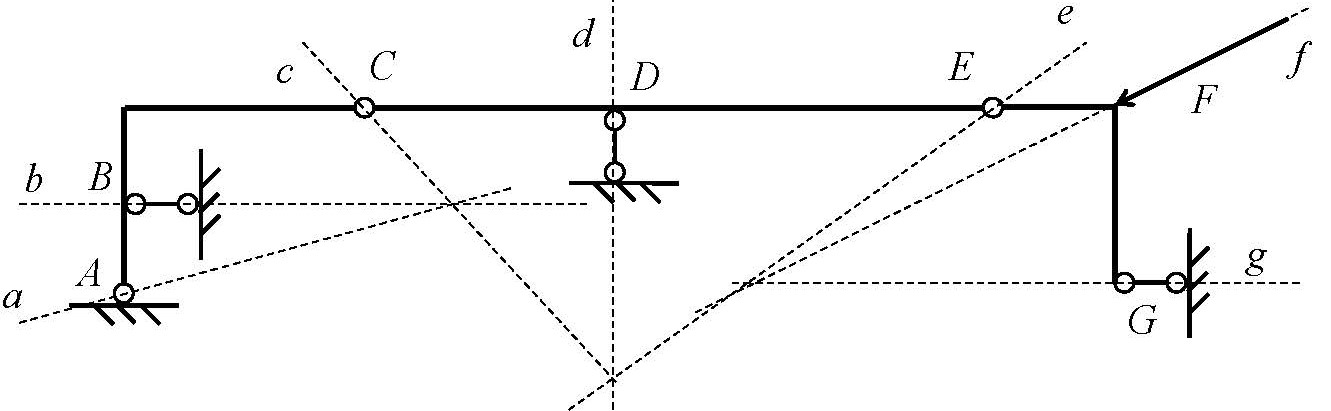
\includegraphics[width=0.5\linewidth]{immagini/1.PARTE4_Pagina_32.1}
\end{figure}

Infine sarà ora la retta \underline{a} ora a dover passare nel punto d'intersezione tra \underline{c}  e \underline{b}:
\[\underline{a} + (\underline{b} + \underline{c}) = 0\]

\begin{figure}[H]
	\centering
	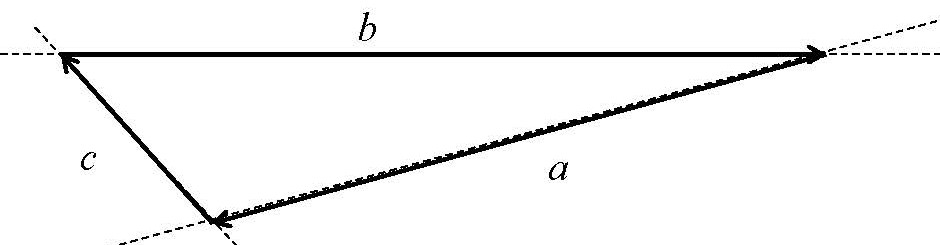
\includegraphics[width=0.4\linewidth]{immagini/1.PARTE4_Pagina_32}
\end{figure}
\newpage
\textbf{Esempio 4} \newline
\begin{figure}[H]
	\centering
	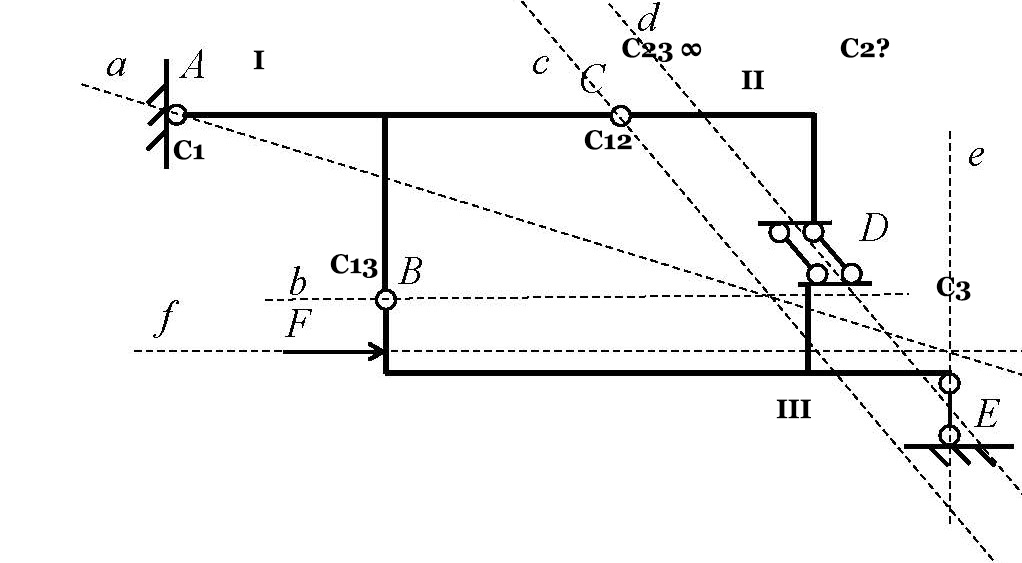
\includegraphics[width=0.5\linewidth]{immagini/1.PARTE4_Pagina_33.1}
\end{figure}
\[\underset{9}{3t} - \underset{9}{s} = 0\]
Si cominci a considerare i centri assoluti: $C_1$ se esiste coincide con $A$, per $C_2$ non ho informazioni mentre $C_3$ se esiste appartiene alla retta $e$.

I centri relativi sono $C_{12}$ coincidente con $C$, $C_{23}$ all'infinito appartenente alla retta $d$ mentre $C_{13}$ coincide con $B$. \newline 

Ebbene, si vede benissimo che nessun centro relativo è allineato: non esiste allineamento tra due punti propri ed uno improprio.

 Non essendoci allora moto relativo è come se i tre corpi si muovessero insieme, come se potessi considerare la struttura unica. 

In più, i tre centri di spostamento assoluto anch'essi non sono allineati e allora il corpo nella sua totalità è fermo. \newline 

In generale, se si dimostra che i centri di spostamento relativi non sono allineati, la struttura diviene unica e ci si concentra sui centri si spostamento assoluti, che se non saranno allineati, ci porteranno a concludere che la struttura è ferma. \newline 

Perciò in questo caso:
\[i=l=0\]
E la struttura è isostatica, si può applicare il metodo grafico. 
\[\begin{cases}
	1. ~ a + b+ c = 0\\
	2. ~ c + d  = 0 \\
	3. ~ d + e+ f +b = 0 \\
	\text{Globale:} ~ a + e + f = 0
\end{cases}\]
Dall'equilibrio globale si trova che $a$ passa per l'intersezione tra $e$ ed $f$.

Dall'equilibrio del secondo copro invece si nota che $c$ e $d$ sono parallele e condurranno a reazioni vincolari parallele di modulo opposto. 

Dall'equilibrio del primo corpo si trova che $b$ passa nell'intersezione tra $a$ e $c$. 

\begin{figure}[H]
	\centering
	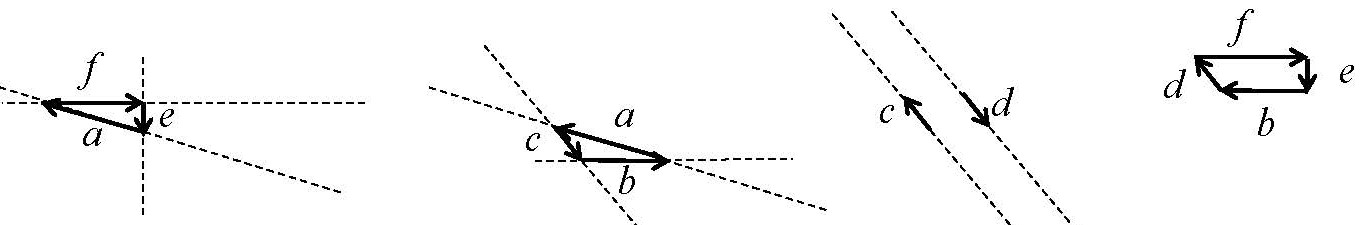
\includegraphics[width=0.6\linewidth]{immagini/1.PARTE4_Pagina_33}
\end{figure}
\newpage
\textbf{Esempio 5} \newline
\begin{figure}[H]
	\centering
	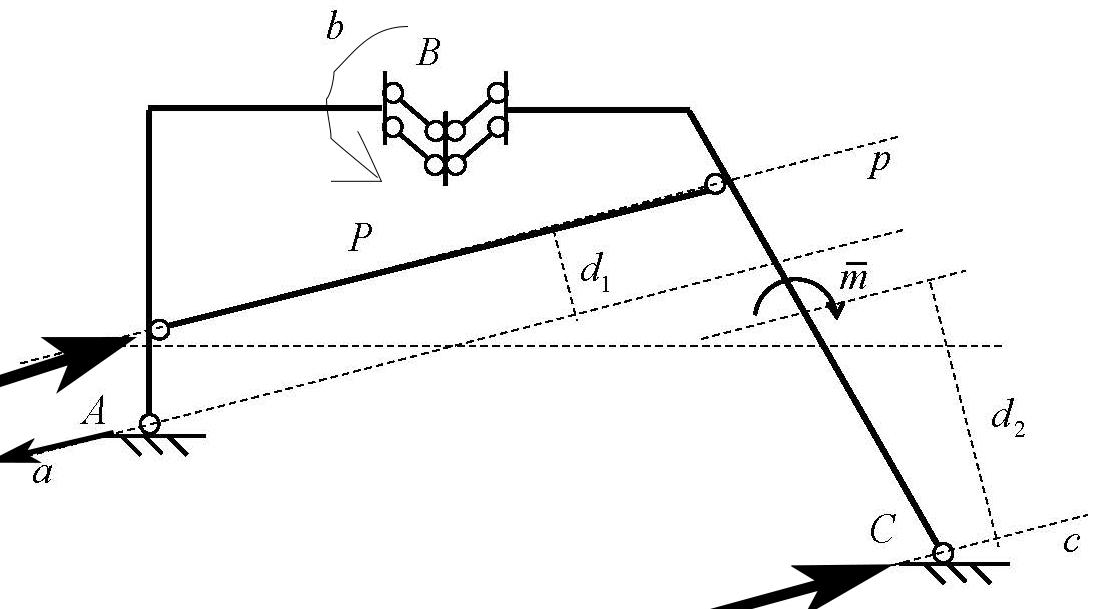
\includegraphics[width=0.5\linewidth]{immagini/1.PARTE4_Pagina_34}
\end{figure}
Una trave incernierata come in figura, piuttosto che essere considerata un terzo corpo, può essere schematizzabile come un pendolo interno.
\[\underset{6}{3t} - \underset{6}{s} = 0\]
La congiungente della retta $C_1C_2$ è diversa dalla direzione del pendolo interno così schematizzato, nessun centro di spostamento è allineato: la struttura è ferma ed isostatica. 
\[i=l=0\]
E posso applicare il metodo grafico. 
\[\begin{cases}
	1. ~ a + b+ p = 0\\
	2. ~ b+ p + m +c  = 0 \\
	\text{Globale:} ~ a + m + c = 0
\end{cases}\]
L'equilibrio del primo corpo è un equilibrio tra due forze ed un momento, tale equilibrio descrive l'azione di una coppia di forze: la retta $a$ sarà parallela alla retta $p$, ma traslata di un $d_1$ atto a verificare l'uguaglianza col momento:
\[a\cdot d_1 = p\cdot d_1 = b \Rightarrow a = p = {b\over d_1}\]
Anche l'equilibrio globale descrive una coppia di forze per cui:
\[a\cdot d_2 = c\cdot d_2 = m \Rightarrow a = c = {m\over d_2} \]
Infine: 
\[ b = a\cdot d_1 =  {m\over d_2}\cdot d_1 \]
In questo modo so solo però dove agiscono le forze e in che modo, ma la loro direzione mi è ignota, allora dall'equilibrio globale so che un momento orario mi genera una coppia di forze antioraria, ora che so la direzione di $a$, $p$ sarà uguale e opposta e la coppia $p,a$ mi descriverà così una coppia oraria equilibrata da un momento $b$ antiorario. 
\newpage

\textbf{Esempio 6} \newline
\begin{figure}[H]
	\centering
	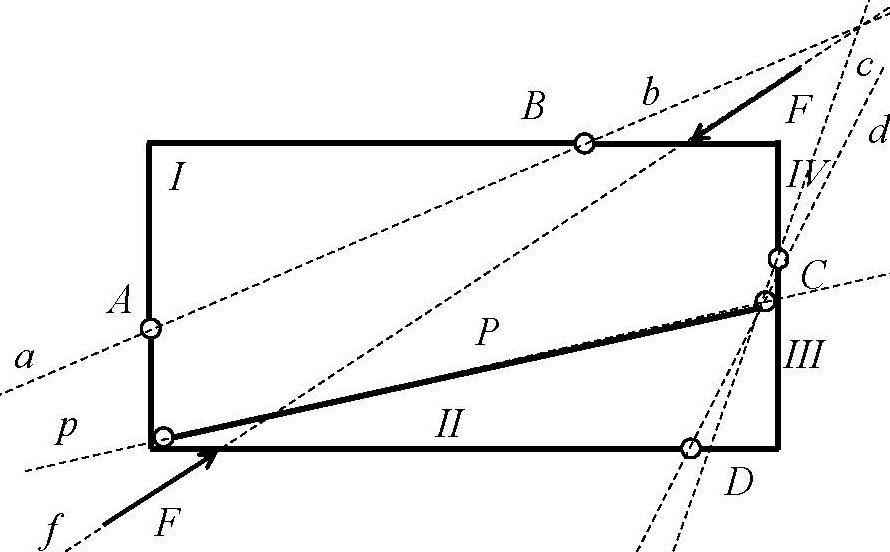
\includegraphics[width=0.5\linewidth]{immagini/1.PARTE4_Pagina_35}
\end{figure}
In questa struttura i corpi sono 5, 4 se si considera la trave interna essere un pendolo interno come nell'esempio precedente.:
\[3t - s = 12 - 9 = 3 \]
Questa struttura non ha applicati vincoli esterni, cosa significa? Che può muoversi e allora $l=1$.

Ci si accorge però nell'impossibilità di avere informazioni su questi vincoli esterni, è necessario fornire arbitrariamente le informazioni per individuarli, e di quante informazioni ho bisogno per individuare un punto sul piano? Di $x$ ed $y$. 
Equivalentemente, se ci si accorge che questa struttura sul piano può muoversi come vuole, traslando su $ x, y  $ e ruotare introno a $z$, si giunge facilmente alla conclusione che, per na struttura del genere:
\[ l = 3\]
Perciò si ha, infine: 
\[3t - s = l - i \Rightarrow 3 = 3 - i \Rightarrow i = 0 \]
La struttura è iperstatica e si può applicare il metodo grafico.
\[\begin{cases}
	1. ~ a + b = 0\\
	2. ~ a + p +f + d  = 0 \\
	3. ~ p + c + d = 0 \\
	4. ~ b + c + f = 0 \\
	\text{Globale:} ~ f  + f = 0
\end{cases}\]
Dall'equilibrio del primo corpo si nota che $a$ e $b$ si equilibrano: hanno lo stesso modulo e la stessa retta d'azione. 

Dall'equilibrio del quarto corpo $b,f,c$ concorrono nello stesso punto.

\begin{figure}[H]
	\centering
	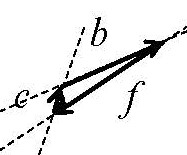
\includegraphics[width=0.15\linewidth]{immagini/1.PARTE4_Pagina_35.1}
\end{figure}
\newpage
Dall'equilibrio del terzo corpo $p,c,d$ concorrono nello stesso punto. 

\begin{figure}[H]
	\centering
	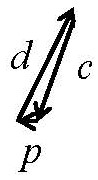
\includegraphics[width=0.06\linewidth]{immagini/1.PARTE4_Pagina_35.2}
\end{figure}

Dall'equilibrio globale si vede poi come si sta applicando una forza uguale e opposta sulla stessa retta d'azione ad un corpo libero nel piano, ciò che è possibile fare è trovare un set di reazioni vincolari interne in equilibrio  con queste due forze:
\[F\cdot s - F\cdot s = 0\]
Applicando la stessa forza la struttura si sposterà della stessa quantità. 

Per strutture del genere non è necessario perciò studiare l'equilibrio globale. 

\begin{figure}[H]
	\centering
	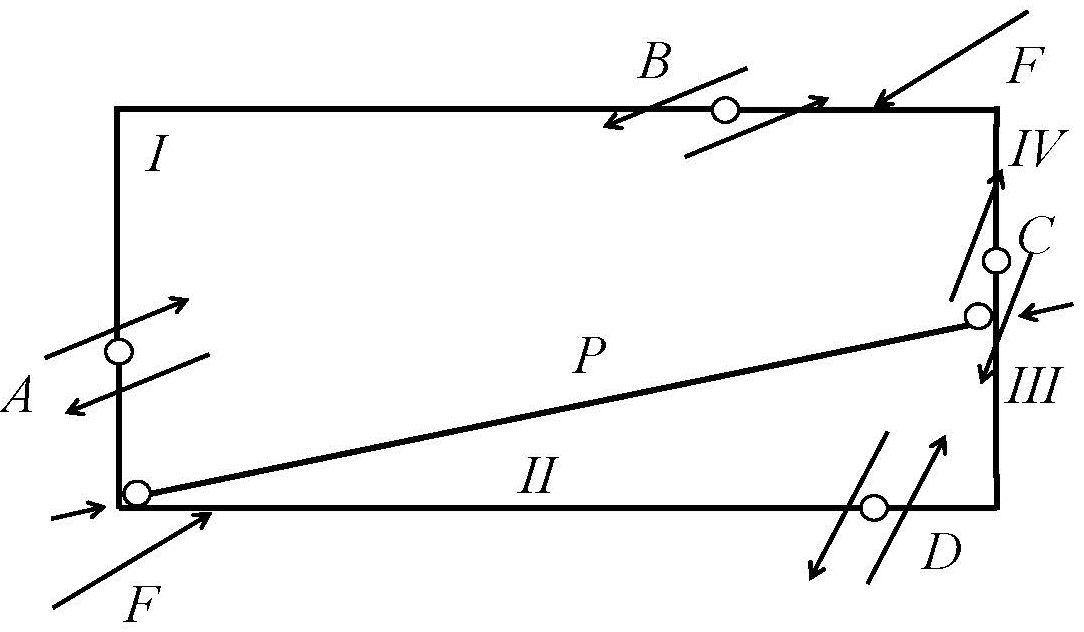
\includegraphics[width=0.5\linewidth]{immagini/1.PARTE4_Pagina_36}
\end{figure}

Notare come la reazione di P, frecce in nero, stia cercando di mantenere la posizione di quegli estremi. \newline

 \begin{center}
 	\textbf{UN PENDOLO SOGGETTO A TRAZIONE SI CHIAMA TIRANTE, UN PENDOLO SOGGETTO A COMPRESSIONE SI CHIAMA PUNTONE}
 \end{center}

 
	\newpage
	{\Large \textbf{Note}}
%	\vfill
%	\begin{tcolorbox}[height=4.5cm]
%		This box has a height of 1cm.
%	\end{tcolorbox}
	
\end{adjustwidth}
\end{document}